\documentclass{article}

\usepackage[utf8]{inputenc} % allow utf-8 input
\usepackage[T1]{fontenc}    % use 8-bit T1 fonts
\usepackage{hyperref}       % hyperlinks
\usepackage{url}            % simple URL typesetting
\usepackage{booktabs}       % professional-quality tables
\usepackage{amsfonts}       % blackboard math symbols
\usepackage{nicefrac}       % compact symbols for 1/2, etc.
\usepackage{microtype}      % microtypography
\usepackage{xcolor}         % colors
\usepackage{algorithm}
\usepackage{algpseudocode}
\usepackage{amsmath}
\usepackage{makecell}
\usepackage{pgfplots}
\pgfplotsset{compat=1.17}

\usepackage[final]{main}    % Use the final version of the NeurIPS style

\title{Convolutional Neural Networks in 1.58 Bits}

\author{%
  Dario Cazzani \\
  Collaboration AI Team \\
  Cisco Systems \\
  \texttt{dariocazzani@gmail.com} \\
  \texttt{dcazzani@cisco.com} \\
  \And
  Aleksandr Yeganov \\
  Collaboration AI Team \\
  Cisco Systems \\
  \texttt{ayeganov@gmail.com} \\
  \texttt{ayeganov@cisco.com}
}

\begin{document}

\maketitle

\begin{abstract}
The rapid evolution of large language models (LLMs) towards 1-bit architectures has proven effective in reducing their energy and memory footprint. Landmark studies such as BitNet \cite{wang2023bitnet} and "The Era of 1-bit LLMs: All Large Language Models are in 1.58 Bits" \cite{ma2024era} have paved the way for significant efficiency improvements without compromising performance. Extending these innovations, this paper explores the application of 1.58-bit quantization to convolutional neural networks (CNNs), specifically examining MobileNet and ResNet architectures. We conduct extensive experiments on well-known datasets including CIFAR-10/100, MNIST, and CelebA, analyzing the impacts of reduced bit-width on these networks. Our results reveal that while the performance of some models slightly decreases, the efficiency gains are substantial. We complement our study with open-source code to foster reproducibility and enable further academic and practical advancements.
\end{abstract}

\section{Introduction}

The escalating computational demands of large language models necessitate continuous innovation to optimize their architecture for reduced energy consumption and memory usage without sacrificing performance. Recent advances have demonstrated the potential of 1-bit architectures in achieving these goals, with studies such as BitNet \cite{wang2023bitnet} and "The Era of 1-bit LLMs: All Large Language Models are in 1.58 Bits" \cite{ma2024era} providing foundational frameworks that balance scalability and computational efficiency. However, the adaptation of these techniques to convolutional neural networks (CNNs) presents unique challenges, particularly in maintaining performance metrics across diverse tasks and datasets. This research extends the 1.58-bit quantization approach, previously confined to linear models, to prominent CNN architectures such as MobileNet and ResNet. Through rigorous testing on CIFAR-10/100, MNIST, and CelebA datasets, we offer a comprehensive evaluation of how CNNs perform under the constraints of reduced bit-width, providing valuable insights into the potential and limitations of further bit reduction in neural network architectures. This paper not only details our findings but also contributes to the community by releasing our experimental framework as open-source software, ensuring that our results are reproducible and that the methodologies employed can be further explored and enhanced by the research community.


The significance of this research extends beyond the technical advancements, as it addresses the pressing need for environmentally sustainable and inclusive AI development. By exploring the potential of 1.58-bit quantization in convolutional neural networks, we aim to contribute to a more energy-efficient and equitable AI ecosystem. Our work has the potential to enable the widespread adoption of AI technologies in resource-constrained settings, such as edge devices or developing regions, and to reduce the environmental impact of large-scale AI deployments, aligning with the United Nations' Sustainable Development Goals (SDGs) related to climate action and digital inclusion.

\section{Methodology}

The core innovation of our methodology lies in adapting the 1.58-bit quantization technique, originally applied to linear layers, to convolutional neural networks. The convolutional operation, fundamentally linear in its application of weights to inputs, permits a direct transposition of the quantization techniques used for linear models.

The quantization approach is based on the absmean quantization function described in "The Era of 1-bit LLMs: All Large Language Models are in 1.58 Bits" \cite{ma2024era}, which involves scaling the weight matrix by its average absolute value, then rounding each value to the nearest integer among \{-1, 0, +1\}.

The following pseudocode details the quantization function for both linear and convolutional layers:
\begin{algorithm}
  \caption{Quantization Function}
  \begin{algorithmic}[1]
  \Function{QuantizeWeights}{$weights$, $gamma$, $epsilon$}
      \State $scaled\_weights \gets weights / (gamma + epsilon)$
      \State $rounded\_weights \gets \Call{Round}{scaled\_weights}$
      \State $bin\_weights\_no\_grad \gets \Call{Clamp}{rounded\_weights, -1, 1}$
      \State \Return $(bin\_weights\_no\_grad - weights).detach() + weights$
  \EndFunction
  \end{algorithmic}
  \end{algorithm}


Both layer types utilize the \textit{weights\_gamma} factor, defined as $\gamma$, to scale the weights matrix by its average absolute value before rounding:
\[
\gamma = \frac{1}{nm} \sum_{ij} |W_{ij}| \tag{3}
\]
Here, $nm$ represents the total number of weights.

The similarity in handling the weights between the two layer types highlights the universality and adaptability of our quantization approach. The primary difference lies in the type of operation: while \textit{BitLinear} applies a matrix multiplication, \textit{BitConv2d} applies a convolutional filter operation. However, the quantization and dequantization steps remain identical, underscoring the consistency of our approach across different types of neural network layers.

This methodological adaptation is crucial for extending the benefits of 1.58-bit quantization—namely, significant reductions in memory and computational overhead—to a broader range of architectures and applications. The technical contribution of this research lies in demonstrating.

Reference to these equations and their implementation in both types of neural network layers ensures that our approach maintains high efficiency while adapting to the specific demands and operational characteristics of convolutional networks.


\section{Results}

The experimental results presented in this section are derived entirely from automated processes. Each table encapsulating the performance metrics of our models has been generated by executing a series of scripts that run the models, collect outcomes, and perform statistical analysis on these outcomes. This automation ensures that all data is up-to-date and reflects the most recent experimental runs without manual intervention.

To maintain transparency and reproducibility, we have embedded the generation and updating of these results directly into our document workflow. The tables below are inserted into the LaTeX document via a script that parses the output from our experimental pipeline. This method guarantees accuracy and efficiency, allowing us to dynamically update our findings as new data becomes available or as additional experiments are conducted.

\subsection{Comparison of BitNet and FloatNet}

In the ensuing tables, we present a comparative analysis of performance metrics for two distinct configurations: BitNet, which employs the innovative 1.58-bit quantization strategy, and FloatNet, the conventional architecture that operates with standard floating-point precision. This side-by-side evaluation spans a variety of architectures and datasets, focusing on the mean accuracy and its standard deviation as a measure of performance consistency and computational robustness. By contrasting these models, we aim to shed light on the efficiency and efficacy trade-offs introduced by adopting lower-precision computations in BitNet as compared to the unquantized baseline established by FloatNet.


% BEGIN_TABLE
\begin{table}[h]
\centering
\begin{tabular}{|c|c|c|c|c|}
\Xhline{2\arrayrulewidth}
\textbf{Architecture} & \textbf{Dataset} & \textbf{Type} & \textbf{Mean Accuracy (\%)} & \textbf{Std Dev (\%)} \\
\Xhline{2\arrayrulewidth}
feedforward & mnist & BitNet & 96.31 & 0.03 \\
feedforward & mnist & FloatNet & \textbf{96.53} & 0.09 \\
\Xhline{2\arrayrulewidth}
lenet5 & mnist & BitNet & 98.88 & 0.09 \\
lenet5 & mnist & FloatNet & \textbf{98.99} & 0.06 \\
\Xhline{2\arrayrulewidth}
\end{tabular}
\caption{Experimental Results Comparing BitNet and FloatNet across various architectures and datasets.}
\label{tab:results}
\end{table}

\begin{figure}[h]
\centering
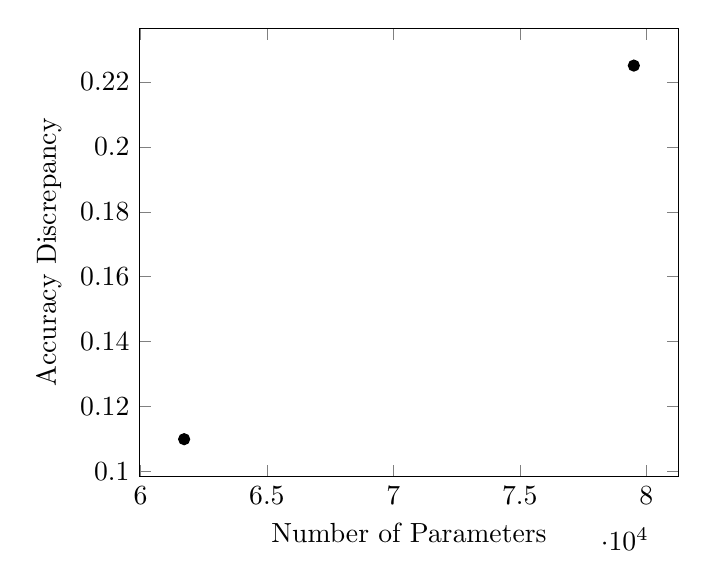
\begin{tikzpicture}
\begin{axis}[
xlabel={Number of Parameters},
ylabel={Accuracy Discrepancy},
]
\addplot[only marks] coordinates {
(79510, 0.22499999999999432) (61728, 0.11000000000001364) 
};
\end{axis}
\end{tikzpicture}
\caption{Correlation between number of parameters and accuracy discrepancy for BitNet and FloatNet.}
\label{fig:discrepancy_plot}
\end{figure}

% END_TABLE

\subsection{Discussion}

The results indicate significant variations in performance, influenced by model architecture and dataset complexity. These variations are discussed in detail, focusing on the trade-offs between computational efficiency and model accuracy. We explore the implications of these findings for practical applications and further research in the field of low-bit neural networks.



\bibliographystyle{plain}
\bibliography{references}

\end{document}
